\documentclass[11pt]{template}

\member{1}{Noemi Bongiorni}{noemibongiorni}{278173}
\member{2}{Alessandro Pedone}{alepedone}{273814}
\member{3}{Simone Licciardi}{simonelicciardi}{214875}
\member{4}{Federico Maria Riva}{feder}{280447}

\teamname{NoPainNoTrain}

\begin{document}

\head

\begin{multicols}{2}
       
\section{Introduction}
This project aims to classify RGB images of blood cells among eight disjoint classes (\emph{basophil [0], eosinophil [1], erythroblast [2], immature granulocytes [3], lymphocyte [4], monocyte [5], neutrophil [6], platelet [7]}) through a CNN.

\section{Problem Analysis}

To assess the task, we perform a statistical and visual inspection of the dataset, determining its relevant characteristics and noticing several outliers.

\textbf{Dataset inspection.}
The dataset consists of a \texttt{(13759, 96, 96, 3)} tensor, the 3-channel RGB images, and a \texttt{(13759,)} tensor of labels. 

\textbf{Main challenges.}
Visual inspection reveals the main learning challenges. Images differ by \textit{details}, not global pattern; formally, high-frequency differences are more important than low-frequency ones.
%(see Figure \ref{fig:general_data})
Moreover, there is an \emph{unbalanced} distribution of  samples among classes
% (see Figure \ref{fig:classes_histogram})
and some images are corrupted by the \textit{superposition} of another image (see Figure \ref{fig:filters1}).
Some other images are corrupted by \textit{colour filtering} (see Figure \ref{fig:filters2}).
To address the above, we preprocess the dataset by detecting and \textbf{removing superpositioned images} (resulting in a clean \texttt{(11959, 96, 96, 3)} tensor), while we leave blue-filtered ones untouched due to difficult detection and overall small impact (indeed, the filtering preserves the high-frequency changes). The latter seems to account for 2\% of the database.
We also choose high-pass filter layers in the model, and add class weights to contrast the other highlighted challenges.

\textbf{Initial assumptions.}
We assume that for each image there is no ambiguity on its unique class (equivalently, that either the model is correct, or is mistaken), that all mistakes weight the same towards our downstream tasks, that the images have no preferred orientation and that zoom is constant. 
%\newpage
% \begin{figure}[H]
%     \centering
%         \begin{subfigure}{\linewidth} % Adjust width to fit the column
%             \centering
%             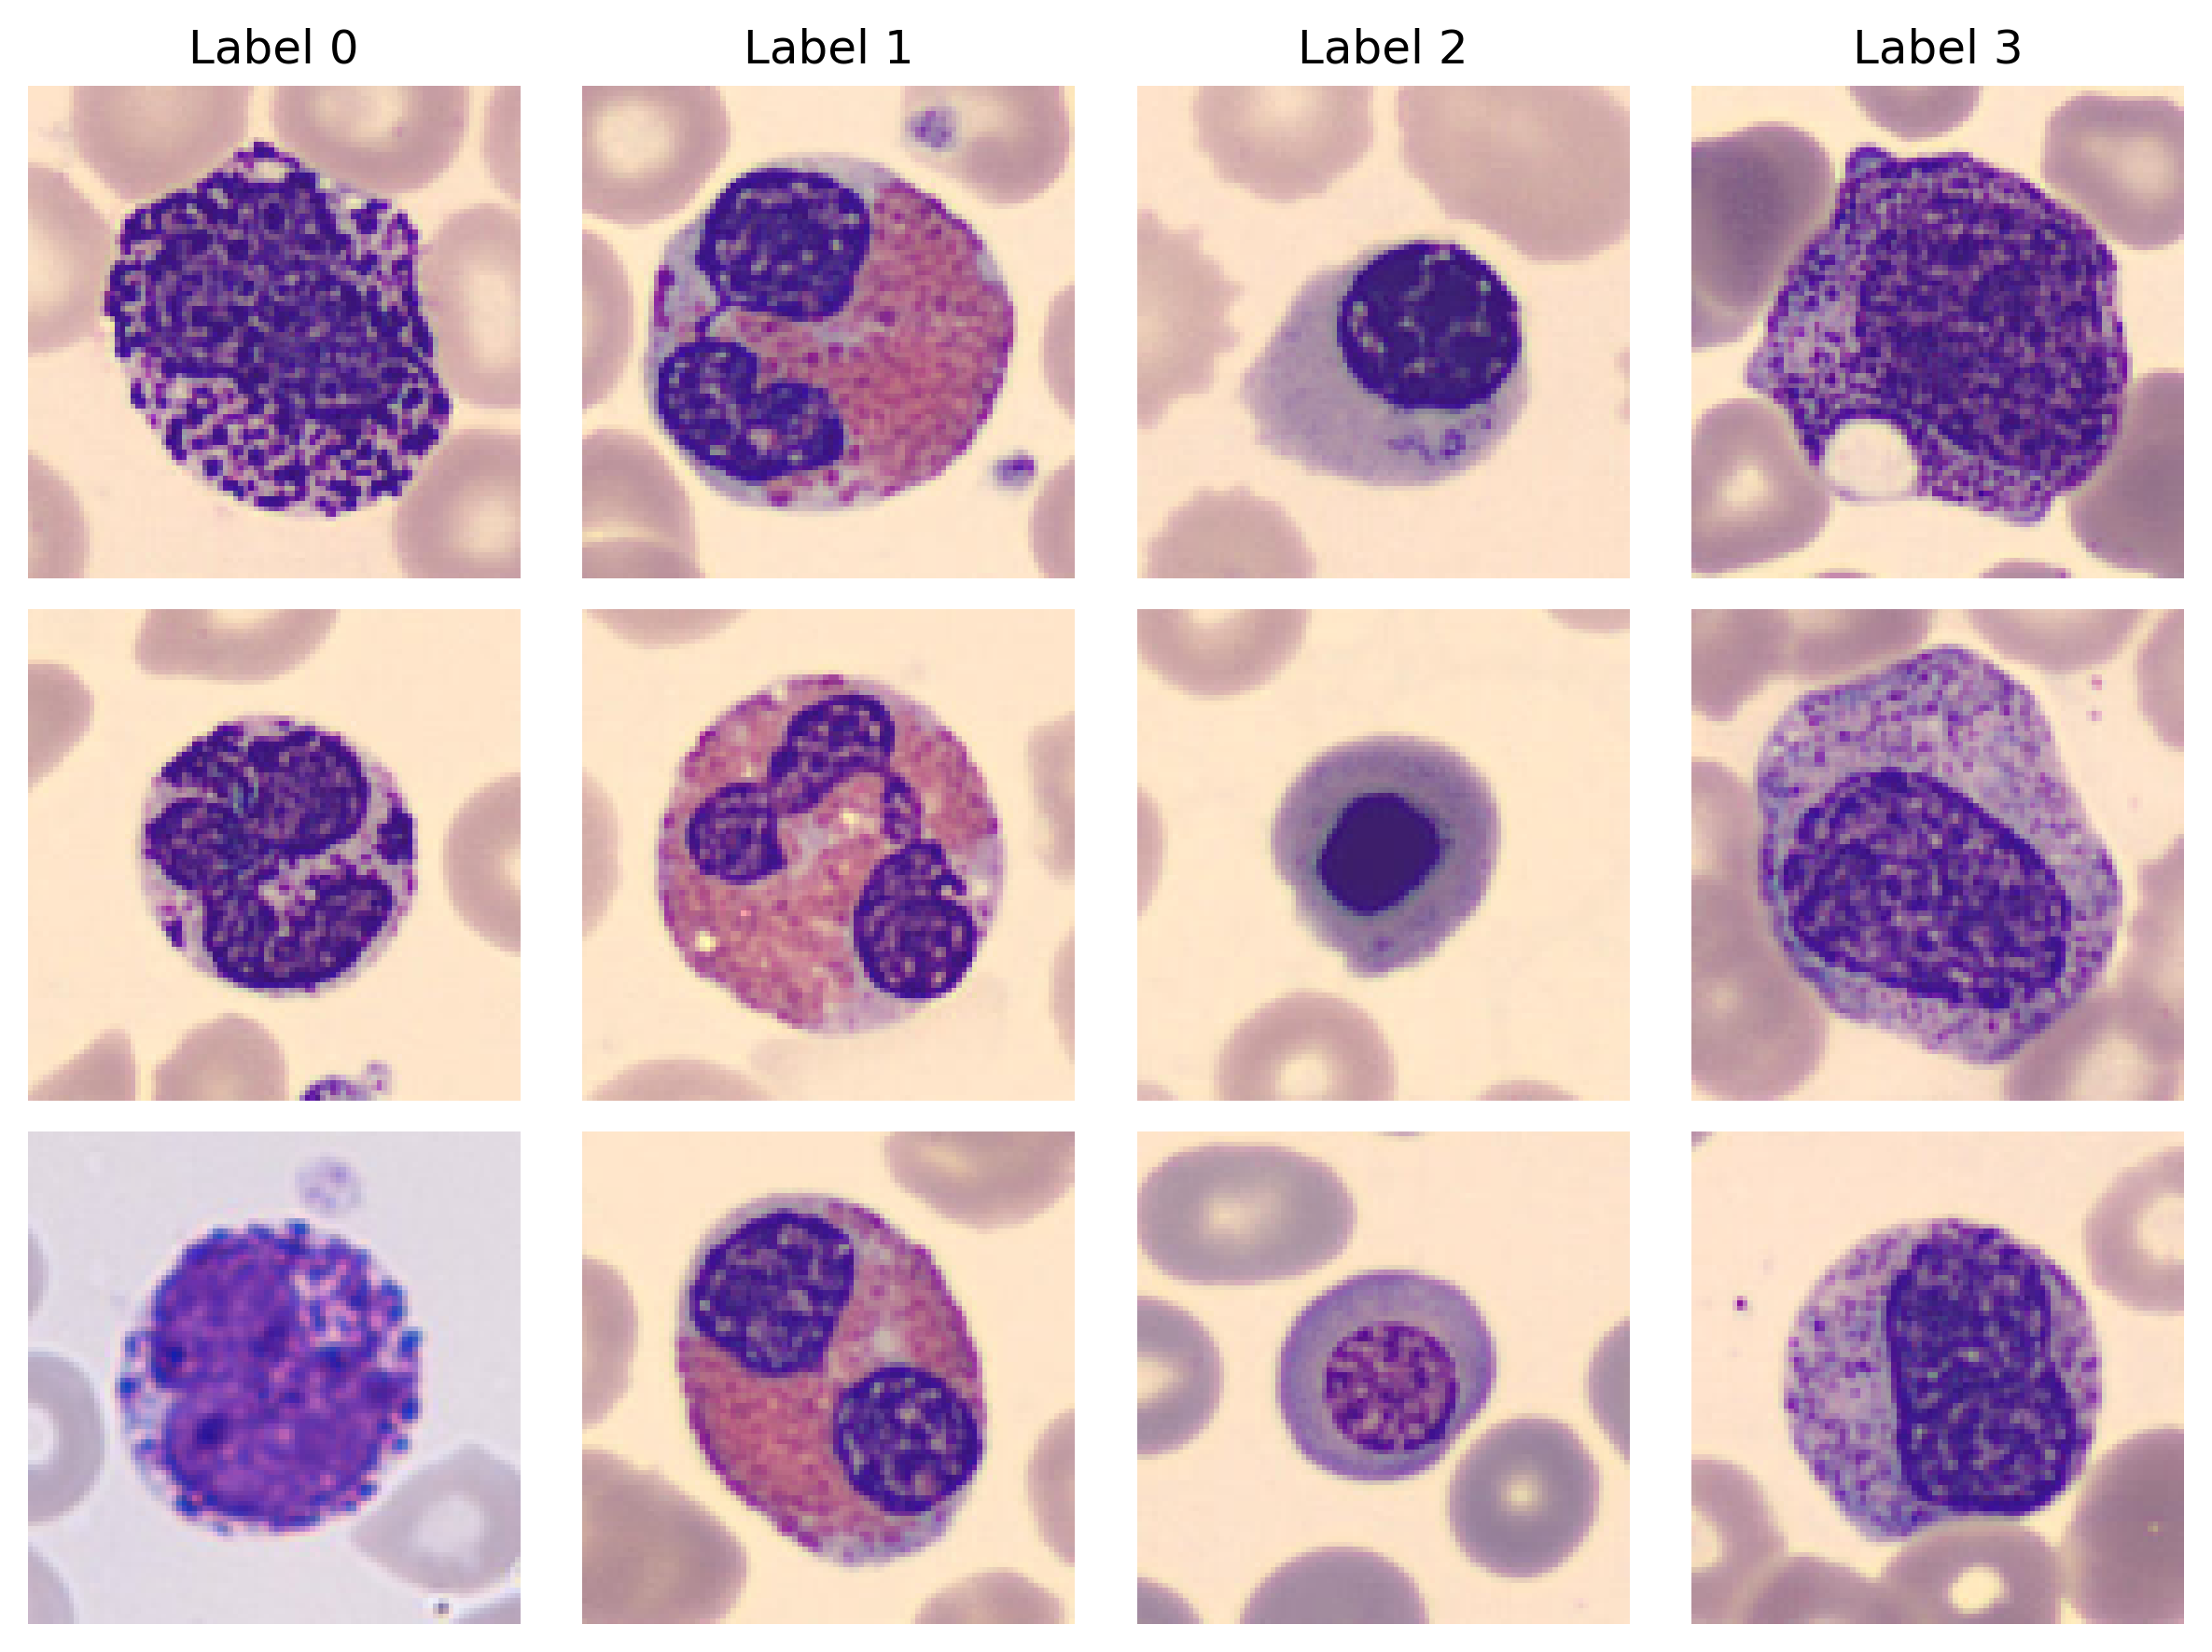
\includegraphics[width=\linewidth]{assets/image_grid_start.png} % Replace with the first part of your image
%             \caption{Classes from 0 to 3 (processed database).}
%             \label{fig:general_data1}
%         \end{subfigure}
%     \vspace{2mm} % Optional vertical spacing between parts
%     % Second part of the image
%         \begin{subfigure}{\linewidth}
%             \centering
%             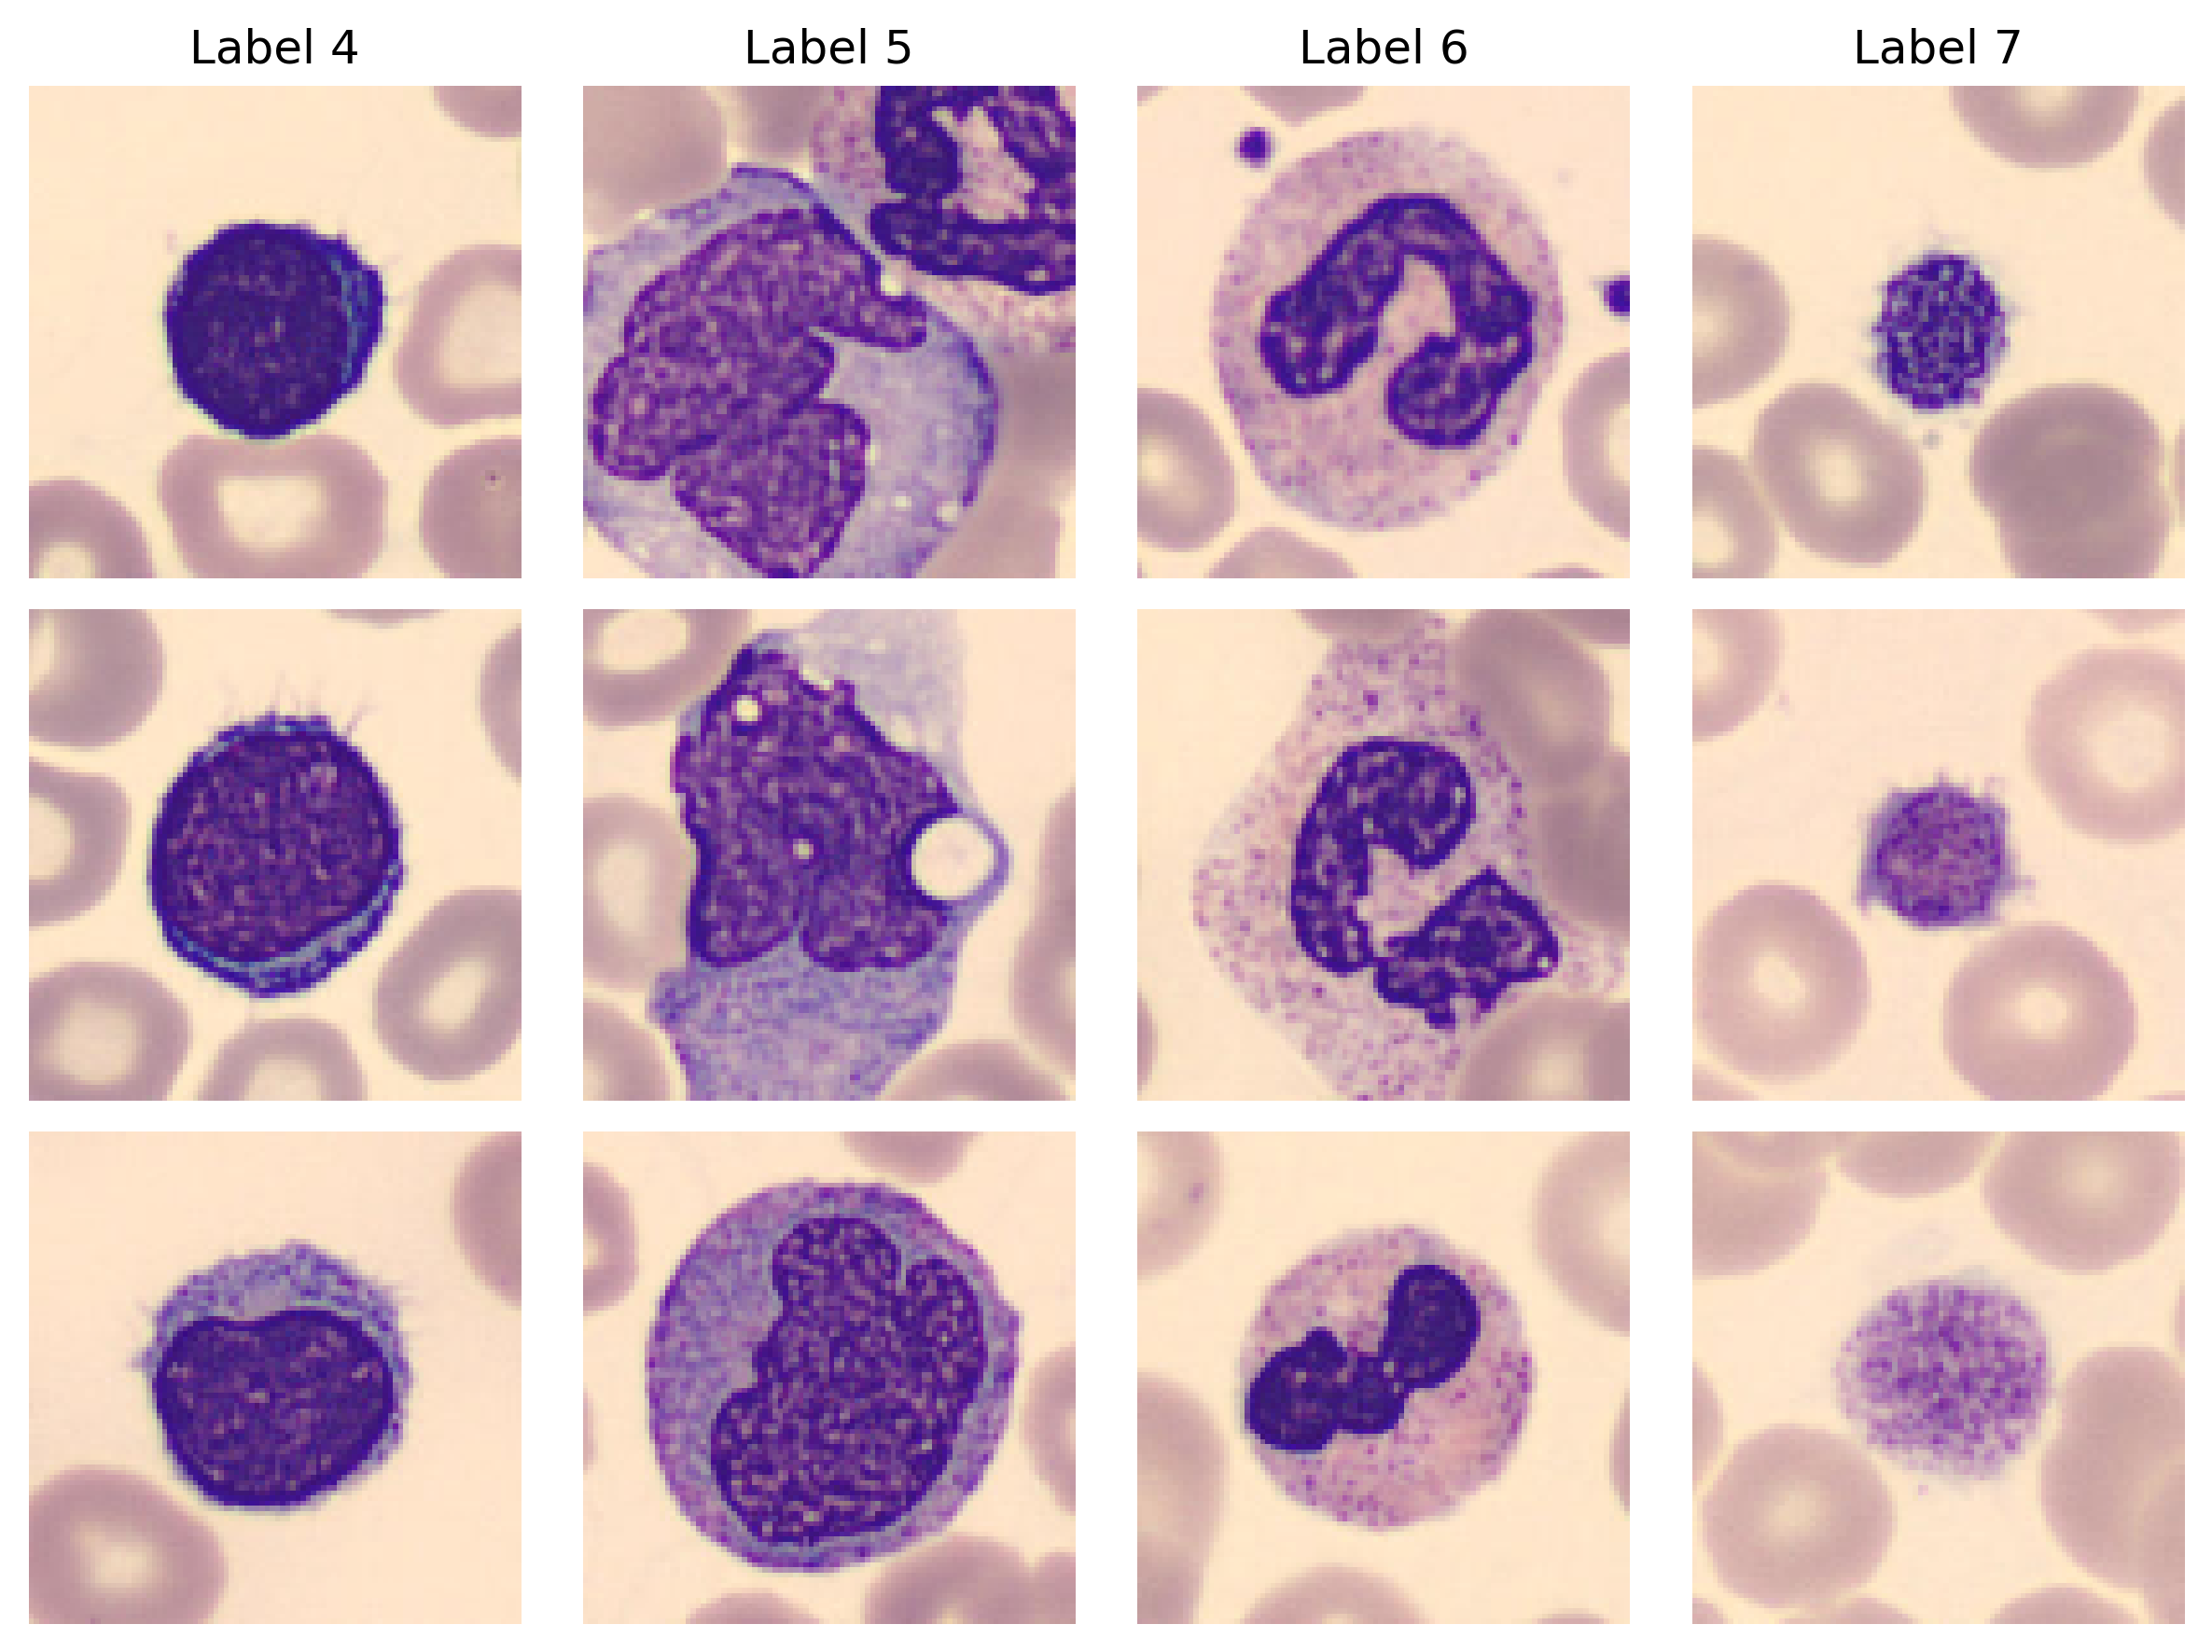
\includegraphics[width=\linewidth]{assets/image_grid_end.png} % Replace with the second part of your image
%             \caption{Classes from 4 to 7 (processed database).}
%             \label{fig:general_data2}
%         \end{subfigure}
%     \caption{Processed database random samples.}
%     \label{fig:general_data}
% \end{figure}
\begin{figure}[H]
        % \begin{subfigure}{\linewidth}
        %     \centering
        %     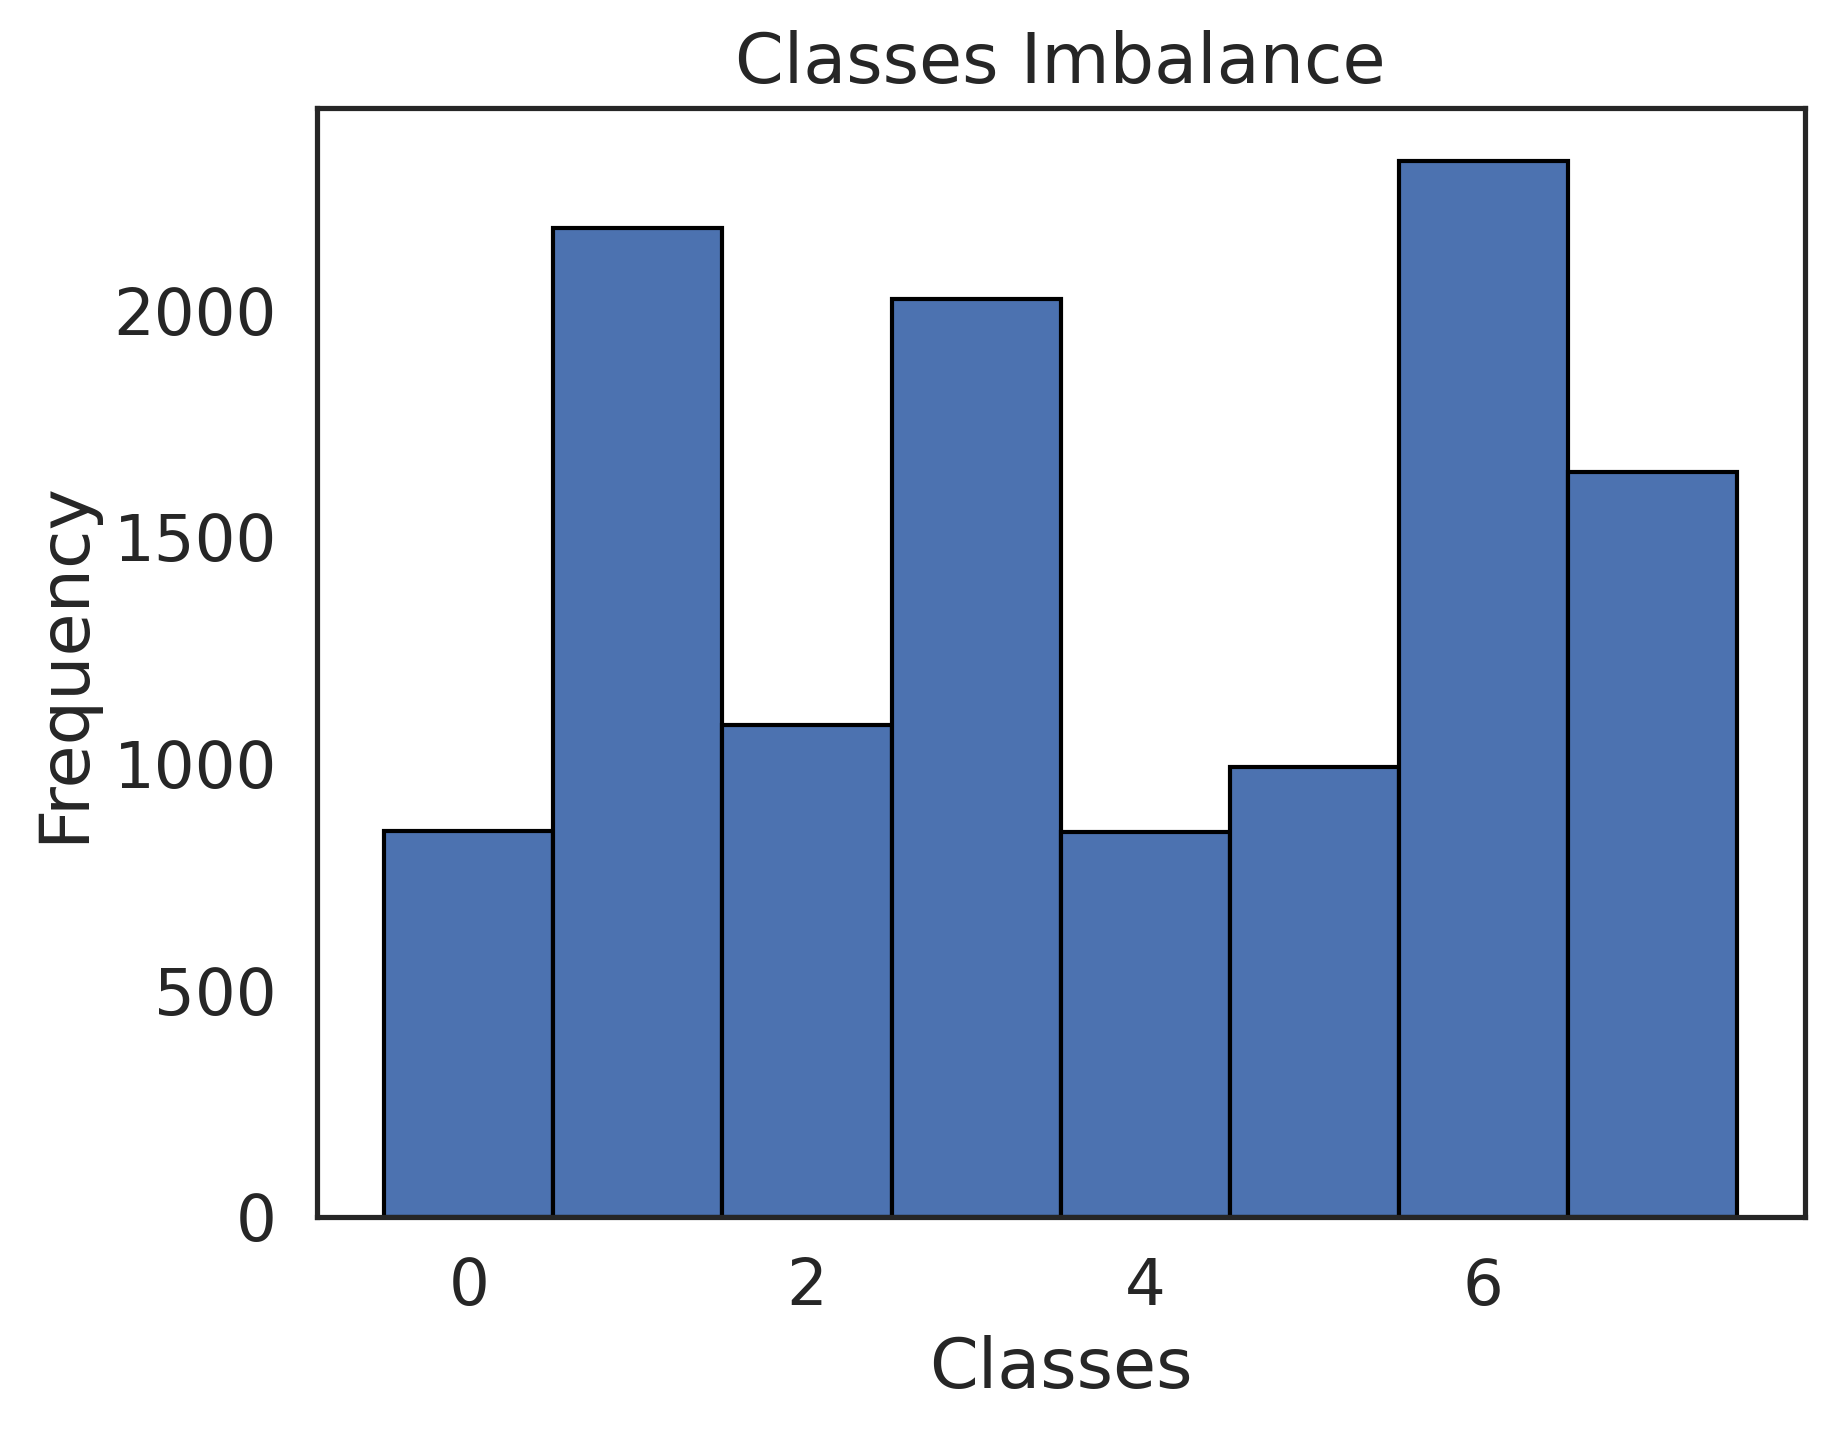
\includegraphics[width=\linewidth]{assets/classes_histogram.png}
        %     \caption{Classes numerosity (processed database).}
        %     \label{fig:classes_histogram}
        % \end{subfigure}
        \begin{subfigure}{\linewidth}
            \centering
            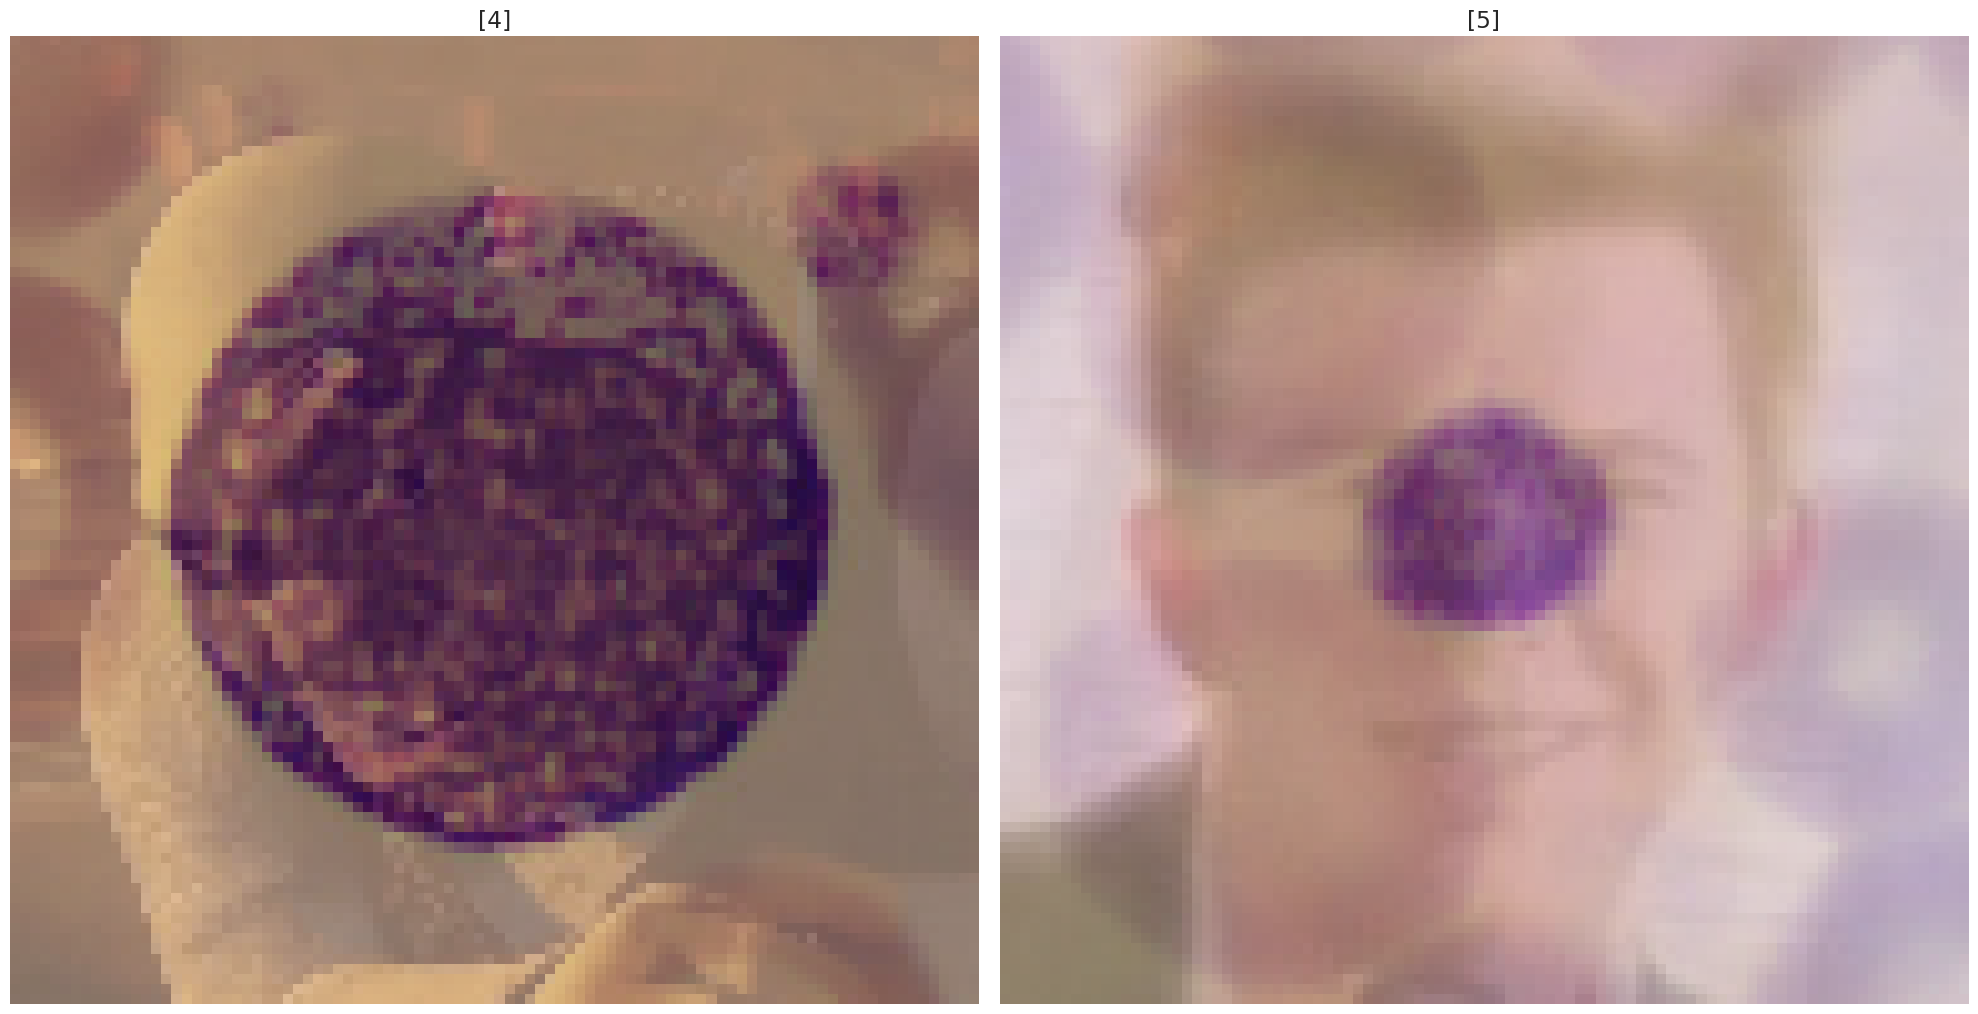
\includegraphics[width=\linewidth]{assets/outliers.png}
            \caption{Images with superposition noise.}
            \label{fig:filters1}
        \end{subfigure}
        \begin{subfigure}{\linewidth}
            \centering
            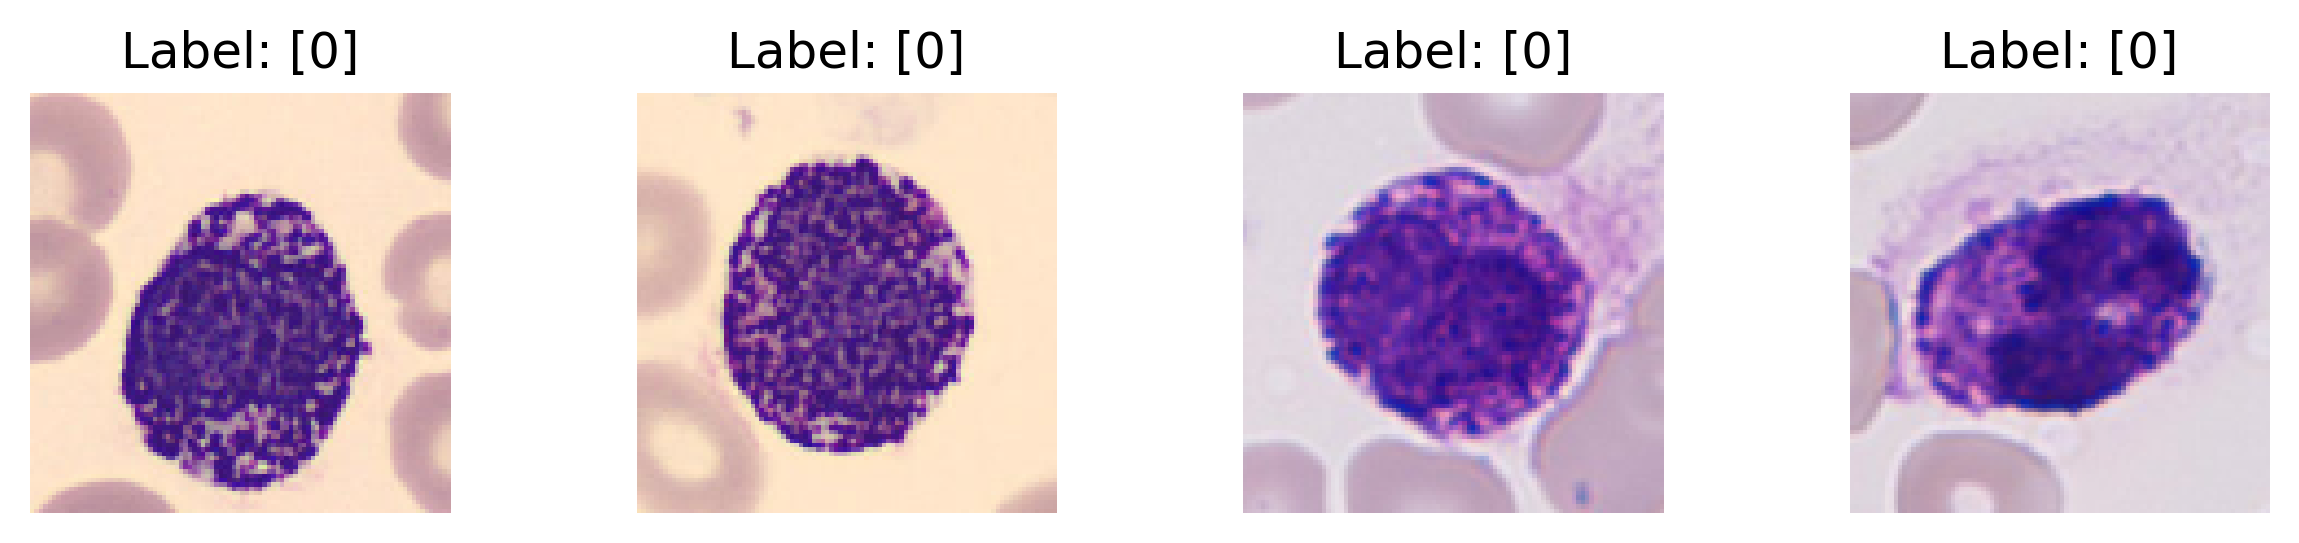
\includegraphics[width=\linewidth]{assets/blue_filter.png}
            \caption{In-class comparison between standard images (left) and blue filtered ones (right).}
            \label{fig:filters2}
        \end{subfigure}
\end{figure}
                
\section{Method}
To develop our solution, we split the filtered dataset into test (20\%), validation (8\%) and training (72\%) sets. We fine-tune hyperparameters, such as the number of \textbf{epochs, batch size, learning rate} (including strategies like reducing the learning rate on plateaus), and \textbf{patience} levels for early stopping. And we implement mixed precision, to balance numerical stability and speed of operations. 
We choose \textbf{categorical cross-entropy} as the loss function, which aligns with evaluation metrics of the external assessment. In order to mitigate overfitting, we use \textbf{early stopping, regularization, dropout} and weight initialization to ensure stable convergence.
We focus on \textbf{data augmentation} too, with the scope of enhancing model robustness, and we utilize standard transformations (flip, rotation, translation, zoom, contrast, etc.), tuning their parameters, so that the they are relevant to the dataset's characteristics and we are avoiding misleading distortions. Additionally, we incorporate \textbf{class weights} to address the imbalance between classes.
The modeling process is devided into two parts, corresponding to two different strategies. First, we design a \textbf{simple architecture} that we can consider a baseline, emphasizes interpretability and allows us to test the effectiveness of some of the already mentioned techniques. Next, we shift our attention towards \textbf{transfer learning} (TL) and \textbf{fine-tuning} (FT) using the available pre-trained networks. The key decisions we make in this step are selecting an appropriate base network, configuring dense layers (e.g., number of units, use of \textbf{batch normalization}, and dropout), specifying input pre-processing and shape and opting for max pooling to capture fine details. For FT, we determine trainable parameters based on a heuristic percentage (between 30\% and 1\%) to balance computational efficiency and feature adaptation.
Finally, we build an \textbf{ensemble} of two neural networks to combine the (complementary) features learned by different architectures and improve overall performance and robustness.

\section{Experiments}
As summarized in Table \ref{tab:1}, we conduct a series of experiments by progressively modifying a baseline CNN architecture to assess the impact of each change on model performance.\newline
\textbf {Baseline} network was trained on the complete dataset comprising 13,759 images. This architecture consists of two blocks, each including a single convolutional layer, followed by a softmax activation layer and a max-pooling layer. While this configuration yields reasonable performance, the results can certainly be improved.\newline
\textbf{Network 1} has the primary modification of training the model on a filtered subset of the dataset (11,959 images). This adjustment consistently improves model performance, demonstrating the benefits of dataset refinement.\newline
\textbf{Network 2} introduces a \textbf{resizing} layer to downscale the input images from 96x96 to 32x32 before the convolutional layers. However, this alteration results in decreased model accuracy, likely due to the loss of critical features caused by the aggressive reduction in spatial resolution.\newline
\textbf{Network 3} incorporates \textbf{LecunNormal} weight initialization and \textbf{L2-norm} regularization for the weights. While these additions don't significantly improve local accuracy, they are hypothesized to stabilize training and potentially enhance generalization.\newline
\textbf{Network 4} adds dropout and batch normalization layers to the architecture. These layers aim to improve generalization and accelerate convergence by reducing overfitting and normalizing feature distributions during training.\newline
When evaluated on CodaBench, none of the models achieves an overall accuracy exceeding 25\%, suggesting suboptimal generalization to unseen test sets. Nevertheless, our experiments provide valuable insights. Specifically: training on the filtered dataset proved beneficial for model performance; downscaling inputs adversely affected accuracy, likely due to the removal of key features; weight initialization, regularization, and the inclusion of dropout and batch normalization, while not yielding noticeable improvements in local accuracy, contributed to better performance on the CodaBench evaluation.
Based on these findings, we retain the most effective techniques and applied them to TL and FT experiments using pre-trained networks to further improve model performance.
As summarized in Table \ref{tab:2} [``/" means that we couldn't upload the model due to CodaBench related issues.], we compare different architectures, using them for TL and FT our model.
The \textbf{percentage of FT} corresponds to the percentage of parameters we decide to unfreeze and re-train for our model. We tested between 1\% and 30\%, reporting in the table the best one for each architecture.
We test the SGD \cite{mandt2018stochasticgradientdescentapproximate}, Adam \cite{yun2024stochgradadamacceleratingneuralnetworks} and \textbf{Lion} \cite{chen2023} optimizers. The best-performing is the latter, with a learning rate schedule from $5\mathrm{e}{-4}$ to $1\mathrm{e}{-5}$ for the TL phase, and from $1\mathrm{e}{-4}$ to $5\mathrm{e}{-6}$ for the FT. The difference in parameters is due to the difference in aim: in the first case we need to train layers from scratch, and so we initially prioritize significant learning steps, while in the second case we are already located near a local minimum and thus the alignment of the source architecture requires smaller stepsizes. 
\FloatBarrier
\begin{table*}[ht]
\centering
\setlength{\tabcolsep}{3pt}
\caption{Comparison on a simple CNN of different choices of parameters/layers/dataset}
\begin{tabularx}{\textwidth}{lYYYc}
    \toprule
    Model & Accuracy & Precision & Recall & F1\\
    \midrule
    Baseline  & 86.59 & 89.71 & 86.59 & 87.17\\

    Network 1 & 94.15 & 94.38 & 94.15 & 94.15  \\

    Network 2 & 91.81 & 91.94 & 91.81 & 91.7 \\

    Network 3 & 91.76 & 91.98 & 91.76 & 91.73  \\

    \textbf{Network 4} & \textbf{91.43} & \textbf{92.02} & \textbf{91.43} & \textbf{91.61} \\
    \arrayrulecolor{black}\bottomrule
\end{tabularx}
\label{tab:1}
\FloatBarrier
\end{table*}
\begin{table*}[ht]
\centering
\setlength{\tabcolsep}{3pt}
\caption{Comparison of different nets for TF and FT}
\begin{tabularx}{\textwidth}{lYYYc}
    \toprule
    Model & Accuracy  & Precision & F1 & FT percentage & & Codabench score & Recall \\
    \midrule
    DenseNet201 &  87.04 & 88.31    &   86.59 & 10    &&   / & 87.04   \\
    \hline
    ConvNeXtTiny   &  96.20    &   96.36     &   96.13    &   1 &  & 53.00    &   96.20\\
    \hline
    ConvNextSmall &  95.74 & 95.88    &   95.76 & 10    &&   64.00 & 95.74   \\
    \hline
    InceptionResNetV2 &  91.39 & 91.76    &   91.43 & 1    &&   48.00 & 91.39   \\
    \hline
    EfficientNetV2B3 &  94.57 & 94.58    &   94.55 & 10    &&   63.00 & 94.57 \\
    \hline
    \textbf{EfficientNetV2S} &  \textbf{93.23}    &   \textbf{93.75}     &   \textbf{93.33}    &    \textbf{10} &&   \textbf{70.00}    &   \textbf{93.23}\\
    \hline
    EfficientNetV2M  & 92.02 & 92.04  & 91.98  & 10    &&   63.00 & 92.02  \\
    \arrayrulecolor{black}\bottomrule
\end{tabularx}
\label{tab:2}
\end{table*}
\noindent Notably, with Lion a schedule increases performance dramatically: its stepsize is fixed and thus cannot converge satisfactorily.
Then we want to choose the number of layer and neurons, for the last dense layers. In the end, a single layer with 64 neurons turns out to be the best choice.
\section{Results}
The \textbf{network} we submitted (CodaBench score of $0.76$) was an ensemble of three models based on the best performing networks: ConvNeXSmall (model1), EfficientNetV2S (model2) and EfficientNetv2B3 (model3). This result demonstrate significant improvements over the baselines, outperforming simpler architectures and basic TF/FT implementations.
\section{Discussion}
\textit{Strengths}: advanced architectures, effective optimization, and an ensemble approach enhanced generalization.
\textit{Weakness}: we couldn't build a model that generalizes well enough so that the local accuracy could match the one on CodaBench.
\textit{Limitation}: we weren't able to test all our ideas to improve our model after the network comparison for TL/FT due to CodaBench not working properly.
\section{Conclusions}
Each team member worked on every task and gave his/her best contribution as follows: Noemi Bongiorni and Alessandro Pedone in architecture design, Simone Licciardi in hyperparameters tuning and ensemble building and Federico Maria Riva in pre-processing and augmentation.
Future areas of development include testing \textbf{additional networks} for TL to improve accuracy by extracting different features, applying \textbf{Grad-CAM} to inspect the model's heat map, and improving image augmentation by allowing \textbf{Keras-CV} library to act directly within the model, after resolving implementation issues.

\nocite{*}
\bibliographystyle{abbrv}
\bibliography{ref}

\end{multicols}
\end{document}